% Generated by code/make_speaker_script.py from docs/speech_script.md -- edit the Markdown, not this file.
\documentclass[10pt]{article}
\usepackage[a4paper,margin=1.2cm,top=1.0cm,bottom=1.0cm]{geometry}
\usepackage[T1]{fontenc}
\usepackage[utf8]{inputenc}
\usepackage{newpxtext,newpxmath}
\usepackage{graphicx,xcolor,newunicodechar,pifont,enumitem}
\usepackage[most]{tcolorbox}
\tcbuselibrary{fitting}
\definecolor{navy}{HTML}{1F3B73}\definecolor{nlred}{HTML}{A93226}\definecolor{grey}{HTML}{7F8C8D}
\definecolor{gold}{HTML}{E0A100}\definecolor{okgreen}{HTML}{2E8B57}
\newunicodechar{−}{\textminus}\newunicodechar{→}{\ensuremath{\rightarrow}}\newunicodechar{≈}{\ensuremath{\approx}}
\newunicodechar{≤}{\ensuremath{\leq}}\newunicodechar{↑}{\ensuremath{\uparrow}}\newunicodechar{€}{\texteuro}
\newunicodechar{λ}{\ensuremath{\lambda}}\newunicodechar{⁴}{\textsuperscript{4}}\newunicodechar{…}{\ldots}\newunicodechar{×}{\ensuremath{\times}}
\setlist[itemize]{leftmargin=1.1em,itemsep=1.5pt,topsep=1pt,parsep=0pt}
\setlist[itemize,2]{leftmargin=1.0em,itemsep=0.5pt,label=--}
\pagestyle{empty}\setlength{\parindent}{0pt}
\tcbset{sbox/.style={enhanced,fit,fit fontsize macros,fit algorithm=fontsize,colback=white,boxrule=0.5pt,arc=2pt,
  left=5pt,right=5pt,top=3pt,bottom=3pt,fonttitle=\bfseries\small,toptitle=1pt,bottomtitle=1pt,before upper=\raggedright}}
\begin{document}

\begin{tcolorbox}[enhanced,colback=navy,colframe=navy,arc=2pt,boxrule=0pt,left=6pt,right=6pt,top=3pt,bottom=3pt]
\color{white}\bfseries\large Page 1/26 · Title\hfill\normalsize about 0:30
\end{tcolorbox}\par\vspace{1pt}
\fcolorbox{black!25}{white}{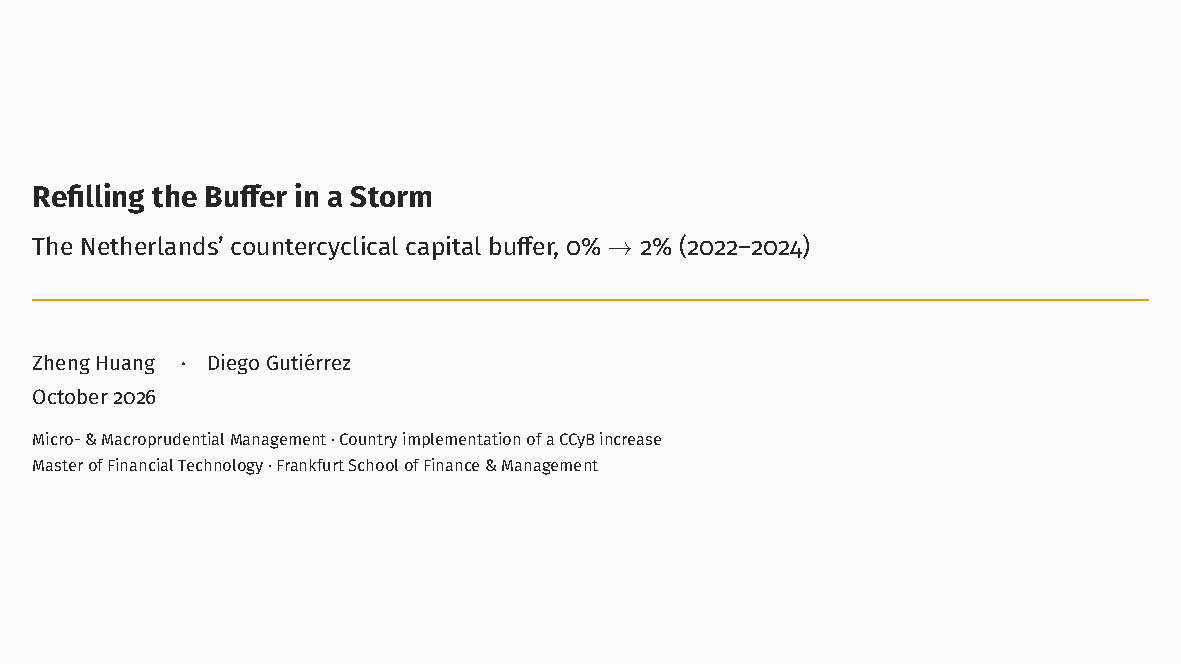
\includegraphics[page=1,width=\dimexpr\linewidth-2\fboxsep-2\fboxrule\relax]{main.pdf}}\par\vspace{4pt}
\begin{tcolorbox}[sbox,width=0.495\linewidth,height=14.6cm,nobeforeafter,box align=top,fit basedim=12.5pt,colframe=navy,colbacktitle=navy!10,coltitle=navy,title=STORY · what to say]
\begin{itemize}
\item Good morning. Our case is the Netherlands.
\item In 2022 and 2023 the Dutch central bank, De Nederlandsche Bank or DNB, raised its countercyclical capital buffer from zero to two percent. We want to explain why it did that, and whether it was a good idea.
\end{itemize}
\end{tcolorbox}\hfill
\begin{tcolorbox}[sbox,width=0.495\linewidth,height=14.6cm,nobeforeafter,box align=top,fit basedim=11pt,colframe=nlred!70,colbacktitle=nlred!8,coltitle=nlred,title=LIKELY CHALLENGES · definitions and logic]
\begin{itemize}
\item[\textcolor{navy}{\textbf{Q}}] \textbf{What is the CCyB, in one sentence?}
\begin{itemize}
\item A capital buffer of 0–2.5\% of risk-weighted assets on domestic exposures that is built up in good times and released in bad times, so banks can absorb losses and keep lending.
\end{itemize}
\item[\textcolor{navy}{\textbf{Q}}] \textbf{Who decides it in the Netherlands?}
\begin{itemize}
\item De Nederlandsche Bank (DNB), the Dutch central bank and designated macroprudential authority. It reviews the rate every quarter.
\end{itemize}
\item[\textcolor{navy}{\textbf{Q}}] \textbf{What exactly changed?}
\begin{itemize}
\item 0\% → 1\% (announced May 2022, binding 25 May 2023) → 2\% (announced 31 May 2023, binding 31 May 2024). It has been held at 2\% since.
\end{itemize}
\end{itemize}
\end{tcolorbox}
\newpage

\begin{tcolorbox}[enhanced,colback=navy,colframe=navy,arc=2pt,boxrule=0pt,left=6pt,right=6pt,top=3pt,bottom=3pt]
\color{white}\bfseries\large Page 2/26 · One-pager\hfill\normalsize about 1:00
\end{tcolorbox}\par\vspace{1pt}
\fcolorbox{black!25}{white}{\includegraphics[page=2,width=\dimexpr\linewidth-2\fboxsep-2\fboxrule\relax]{main.pdf}}\par\vspace{4pt}
\begin{tcolorbox}[sbox,width=0.495\linewidth,height=14.6cm,nobeforeafter,box align=top,fit basedim=12.5pt,colframe=navy,colbacktitle=navy!10,coltitle=navy,title=STORY · what to say]
\begin{itemize}
\item Here is the whole story on one slide. DNB raised the buffer in two steps, to one percent and then to two percent. Yet at both decisions the indicator at the centre of the Basel rules, the credit-to-GDP gap, was deeply negative, so the rulebook said the buffer should be zero.
\item The three columns follow the three questions of the assignment: the environment, the criteria and risks, and the implications.
\item Our verdict is that this was \textbf{normalisation, not tightening}. DNB was refilling an empty buffer, not fighting a credit boom. The price is that the policy relies on DNB's judgement rather than on a rule.
\end{itemize}
\end{tcolorbox}\hfill
\begin{tcolorbox}[sbox,width=0.495\linewidth,height=14.6cm,nobeforeafter,box align=top,fit basedim=11pt,colframe=nlred!70,colbacktitle=nlred!8,coltitle=nlred,title=LIKELY CHALLENGES · definitions and logic]
\begin{itemize}
\item[\textcolor{navy}{\textbf{Q}}] \textbf{Define the credit-to-GDP gap.}
\begin{itemize}
\item Credit to the private non-financial sector as a share of GDP, minus its long-run trend from a one-sided HP filter (λ = 400,000). It is the Basel starting point for setting the CCyB.
\end{itemize}
\item[\textcolor{navy}{\textbf{Q}}] \textbf{What is the Basel buffer guide?}
\begin{itemize}
\item A mapping from the gap to a buffer rate: below 2pp → 0\%; above 10pp → 2.5\%; linear in between. With gaps of −33 and −47pp it gives 0\%.
\end{itemize}
\item[\textcolor{navy}{\textbf{Q}}] \textbf{What do you mean by 'normalisation, not tightening'?}
\begin{itemize}
\item Normalisation means returning the buffer to its planned normal-times level regardless of the cycle. Tightening means raising it because risk is building up. We test which one fits the evidence on page 14.
\end{itemize}
\item[\textcolor{navy}{\textbf{Q}}] \textbf{Isn't raising capital always a tightening?}
\begin{itemize}
\item Not if other requirements are cut at the same time. The 2020 and 2024 cuts in structural buffers roughly offset the CCyB relative to pre-COVID (page 15).
\end{itemize}
\end{itemize}
\end{tcolorbox}
\newpage

\begin{tcolorbox}[enhanced,colback=navy,colframe=navy,arc=2pt,boxrule=0pt,left=6pt,right=6pt,top=3pt,bottom=3pt]
\color{white}\bfseries\large Page 3/26 · March 2020\hfill\normalsize about 1:15
\end{tcolorbox}\par\vspace{1pt}
\fcolorbox{black!25}{white}{\includegraphics[page=3,width=\dimexpr\linewidth-2\fboxsep-2\fboxrule\relax]{main.pdf}}\par\vspace{4pt}
\begin{tcolorbox}[sbox,width=0.495\linewidth,height=14.6cm,nobeforeafter,box align=top,fit basedim=12.5pt,colframe=navy,colbacktitle=navy!10,coltitle=navy,title=STORY · what to say]
\begin{itemize}
\item The story starts in March 2020. When COVID hit, our neighbours reacted within three weeks: eight European countries cut their countercyclical buffers, as the chart shows. Sweden and Norway had been at two and a half percent; Denmark, Ireland and Lithuania at one percent. Buffers built in good times were used exactly as intended.
\item The Netherlands was at \textbf{zero}, the red dot at the bottom. There was nothing to release.
\item So DNB improvised. It cut the systemic buffers of ING, Rabobank and ABN AMRO and postponed a planned floor on mortgage risk weights. This freed about eight billion euros of capital, enough to support up to 200 billion euros of lending. But those buffers were never designed to be released.
\item And DNB made a promise \emph{(pause)}: once things were back to normal, it would rebuild this capital as a two-percent countercyclical buffer.
\end{itemize}
\end{tcolorbox}\hfill
\begin{tcolorbox}[sbox,width=0.495\linewidth,height=14.6cm,nobeforeafter,box align=top,fit basedim=11pt,colframe=nlred!70,colbacktitle=nlred!8,coltitle=nlred,title=LIKELY CHALLENGES · definitions and logic]
\begin{itemize}
\item[\textcolor{navy}{\textbf{Q}}] \textbf{What does 'release' mean legally?}
\begin{itemize}
\item The authority lowers the CCyB rate with immediate effect. The requirement itself falls, so banks can use that capital to absorb losses or lend without breaching any requirement.
\end{itemize}
\item[\textcolor{navy}{\textbf{Q}}] \textbf{If the Dutch CCyB was 0\%, what did DNB release in 2020?}
\begin{itemize}
\item It cut the systemic risk buffers of ING, Rabobank and ABN AMRO (3\% → 2.5/2/1.5\%) and postponed the mortgage risk-weight floor. Together about €8bn, supporting up to €200bn of lending.
\end{itemize}
\item[\textcolor{navy}{\textbf{Q}}] \textbf{Why was that a 'workaround'?}
\begin{itemize}
\item Systemic buffers are structural charges for the size and importance of banks. They are not meant to move with the cycle, so cutting them blurred their purpose. That is why DNB promised to restore the capital as a releasable 2\% CCyB.
\end{itemize}
\item[\textcolor{navy}{\textbf{Q}}] \textbf{Which countries released, and by how much?}
\begin{itemize}
\item Norway 2.5→1\%, Sweden 2.5→0\%, Iceland 2→0\%, Czech Republic 1.75→1\%, Denmark, Lithuania and Ireland 1→0\%, France 0.25→0\%. Belgium and Germany cancelled planned increases (ESRB table).
\end{itemize}
\end{itemize}
\end{tcolorbox}
\newpage

\begin{tcolorbox}[enhanced,colback=navy,colframe=navy,arc=2pt,boxrule=0pt,left=6pt,right=6pt,top=3pt,bottom=3pt]
\color{white}\bfseries\large Page 4/26 · The releasable layer\hfill\normalsize about 1:10
\end{tcolorbox}\par\vspace{1pt}
\fcolorbox{black!25}{white}{\includegraphics[page=4,width=\dimexpr\linewidth-2\fboxsep-2\fboxrule\relax]{main.pdf}}\par\vspace{4pt}
\begin{tcolorbox}[sbox,width=0.495\linewidth,height=14.6cm,nobeforeafter,box align=top,fit basedim=12.5pt,colframe=navy,colbacktitle=navy!10,coltitle=navy,title=STORY · what to say]
\begin{itemize}
\item Why did an empty buffer matter? Because not all bank capital can be used in a crisis.
\item Read the stack from the bottom: first the minimum requirements, then the buffers on top. The red dashed line is the MDA trigger. If a bank falls below it, its dividends and bonuses are restricted automatically, and markets read that as weakness. So in COVID, banks close to this line cut lending rather than use buffers they were formally allowed to use.
\item The countercyclical buffer is different. The authority can switch it off, so the requirement itself falls, with no penalty and no stigma. It is the only truly \textbf{releasable} layer. And while an increase binds only after twelve months, a release is immediate, so the buffer must be filled before a crisis.
\end{itemize}
\end{tcolorbox}\hfill
\begin{tcolorbox}[sbox,width=0.495\linewidth,height=14.6cm,nobeforeafter,box align=top,fit basedim=11pt,colframe=nlred!70,colbacktitle=nlred!8,coltitle=nlred,title=LIKELY CHALLENGES · definitions and logic]
\begin{itemize}
\item[\textcolor{navy}{\textbf{Q}}] \textbf{Define CET1 and RWA.}
\begin{itemize}
\item CET1 (Common Equity Tier 1) is the highest-quality capital: shares and retained earnings. RWA (risk-weighted assets) weight each exposure by its riskiness, so capital ratios are CET1 / RWA.
\end{itemize}
\item[\textcolor{navy}{\textbf{Q}}] \textbf{Walk through the capital stack.}
\begin{itemize}
\item Pillar 1 minimum 4.5\% CET1, then the bank-specific Pillar 2 requirement, then the combined buffer requirement: capital conservation buffer 2.5\%, O-SII/systemic buffer and CCyB. Pillar 2 guidance sits on top and is not binding.
\end{itemize}
\item[\textcolor{navy}{\textbf{Q}}] \textbf{What is the MDA trigger?}
\begin{itemize}
\item The maximum distributable amount. If CET1 falls below the top of the combined buffer requirement, dividends, buybacks and bonuses are automatically restricted.
\end{itemize}
\item[\textcolor{navy}{\textbf{Q}}] \textbf{Buffers are 'usable' anyway; why do banks not use them?}
\begin{itemize}
\item Falling below the MDA trigger means payout limits, market stigma and rating pressure. COVID evidence shows banks close to the trigger cut lending instead (Couaillier et al., 2022). A released CCyB avoids this because the requirement itself falls.
\end{itemize}
\item[\textcolor{navy}{\textbf{Q}}] \textbf{Why is the 12-month lag important?}
\begin{itemize}
\item An increase binds only 12 months after the announcement, but a release is immediate. So the buffer must be filled before a crisis; it cannot be built once the shock arrives.
\end{itemize}
\end{itemize}
\end{tcolorbox}
\newpage

\begin{tcolorbox}[enhanced,colback=navy,colframe=navy,arc=2pt,boxrule=0pt,left=6pt,right=6pt,top=3pt,bottom=3pt]
\color{white}\bfseries\large Page 5/26 · The question\hfill\normalsize about 1:00
\end{tcolorbox}\par\vspace{1pt}
\fcolorbox{black!25}{white}{\includegraphics[page=5,width=\dimexpr\linewidth-2\fboxsep-2\fboxrule\relax]{main.pdf}}\par\vspace{4pt}
\begin{tcolorbox}[sbox,width=0.495\linewidth,height=14.6cm,nobeforeafter,box align=top,fit basedim=12.5pt,colframe=navy,colbacktitle=navy!10,coltitle=navy,title=STORY · what to say]
\begin{itemize}
\item Two years later, in 2022, DNB began to refill the buffer, and the timing looks strange. On the left is the storm: war, record energy prices, 11.6 percent inflation, the first ECB rate hikes and a housing market about to turn. And the Basel indicator said zero. On the right is the decision: one percent, then two percent.
\item Raising capital requirements in a downturn can amplify the cycle. That is exactly the procyclical mistake the buffer was invented to avoid.
\item So our question is: \textbf{was this the wrong moment?} Was DNB tightening into a slowdown, fighting a hidden boom, or doing something else? We answer in three acts, one for each question of the assignment.
\end{itemize}
\end{tcolorbox}\hfill
\begin{tcolorbox}[sbox,width=0.495\linewidth,height=14.6cm,nobeforeafter,box align=top,fit basedim=11pt,colframe=nlred!70,colbacktitle=nlred!8,coltitle=nlred,title=LIKELY CHALLENGES · definitions and logic]
\begin{itemize}
\item[\textcolor{navy}{\textbf{Q}}] \textbf{What is procyclicality?}
\begin{itemize}
\item Policy or behaviour that reinforces the cycle: tighter in bad times, looser in good times. Raising capital in a downturn can force banks to cut lending exactly when the economy needs it.
\end{itemize}
\item[\textcolor{navy}{\textbf{Q}}] \textbf{Why was this moment suspicious?}
\begin{itemize}
\item War, 11.6\% inflation (2022), ECB hikes from July 2022 and a turning housing market, while the Basel indicator said 0\%. On the surface it looks like the procyclical mistake the CCyB was designed to avoid.
\end{itemize}
\item[\textcolor{navy}{\textbf{Q}}] \textbf{How do the three acts map to the assignment?}
\begin{itemize}
\item Act 1 = economic and financial environment; Act 2 = criteria and financial-stability risks; Act 3 = wide-ranging implications.
\end{itemize}
\end{itemize}
\end{tcolorbox}
\newpage

\begin{tcolorbox}[enhanced,colback=navy,colframe=navy,arc=2pt,boxrule=0pt,left=6pt,right=6pt,top=3pt,bottom=3pt]
\color{white}\bfseries\large Page 6/26 · Timeline\hfill\normalsize about 1:00
\end{tcolorbox}\par\vspace{1pt}
\fcolorbox{black!25}{white}{\includegraphics[page=6,width=\dimexpr\linewidth-2\fboxsep-2\fboxrule\relax]{main.pdf}}\par\vspace{4pt}
\begin{tcolorbox}[sbox,width=0.495\linewidth,height=14.6cm,nobeforeafter,box align=top,fit basedim=12.5pt,colframe=navy,colbacktitle=navy!10,coltitle=navy,title=STORY · what to say]
\begin{itemize}
\item Act one is the setting, and it starts with the timeline. In March 2020 DNB cut the systemic buffers and made its promise. In February 2022 it published a framework with two percent as the normal level. In May 2022 it announced one percent, two months before the ECB's first hike. In May 2023 it announced two percent, together with lower buffers for the largest banks, and both became binding in May 2024.
\item Since then DNB has held two percent at every quarterly review. So the path was two equal steps, a year apart, and then a stop. Keep that pattern in mind for our verdict.
\end{itemize}
\end{tcolorbox}\hfill
\begin{tcolorbox}[sbox,width=0.495\linewidth,height=14.6cm,nobeforeafter,box align=top,fit basedim=11pt,colframe=nlred!70,colbacktitle=nlred!8,coltitle=nlred,title=LIKELY CHALLENGES · definitions and logic]
\begin{itemize}
\item[\textcolor{navy}{\textbf{Q}}] \textbf{Announcement date vs binding date?}
\begin{itemize}
\item Banks get 12 months between an increase being announced and having to meet it. So 1\% was announced in May 2022 and binding in May 2023; 2\% announced in May 2023 and binding in May 2024.
\end{itemize}
\item[\textcolor{navy}{\textbf{Q}}] \textbf{Was the increase a response to ECB tightening?}
\begin{itemize}
\item No. The 1\% was announced on 25 May 2022, two months before the ECB's first hike on 21 July 2022, and the path had been promised in 2020.
\end{itemize}
\item[\textcolor{navy}{\textbf{Q}}] \textbf{Why did the systemic risk buffer become an O-SII buffer in December 2020?}
\begin{itemize}
\item CRD V made the O-SII and systemic risk buffers additive, so DNB converted the large banks' systemic risk buffers into O-SII buffers from 29 December 2020.
\end{itemize}
\end{itemize}
\end{tcolorbox}
\newpage

\begin{tcolorbox}[enhanced,colback=navy,colframe=navy,arc=2pt,boxrule=0pt,left=6pt,right=6pt,top=3pt,bottom=3pt]
\color{white}\bfseries\large Page 7/26 · Macro\hfill\normalsize about 0:55
\end{tcolorbox}\par\vspace{1pt}
\fcolorbox{black!25}{white}{\includegraphics[page=7,width=\dimexpr\linewidth-2\fboxsep-2\fboxrule\relax]{main.pdf}}\par\vspace{4pt}
\begin{tcolorbox}[sbox,width=0.495\linewidth,height=14.6cm,nobeforeafter,box align=top,fit basedim=12.5pt,colframe=navy,colbacktitle=navy!10,coltitle=navy,title=STORY · what to say]
\begin{itemize}
\item What did the economy look like? The left panel shows that real GDP was back above its pre-COVID level during 2021, which is the condition DNB's framework sets before rebuilding the buffer.
\item Then the storm arrived. Inflation, in the middle, peaked at 17 percent in September 2022, and on the right the ECB moved its deposit rate from minus half a percent to four percent in fourteen months. DNB warned that higher funding costs could strain the debt of governments, firms and households.
\item So the macro picture argued \textbf{both ways}: build while the economy can take it, or wait because it is weakening.
\end{itemize}
\end{tcolorbox}\hfill
\begin{tcolorbox}[sbox,width=0.495\linewidth,height=14.6cm,nobeforeafter,box align=top,fit basedim=11pt,colframe=nlred!70,colbacktitle=nlred!8,coltitle=nlred,title=LIKELY CHALLENGES · definitions and logic]
\begin{itemize}
\item[\textcolor{navy}{\textbf{Q}}] \textbf{Why does the recovery matter for the decision?}
\begin{itemize}
\item DNB's framework only builds the buffer once the economy has recovered from a crisis (phase 1 → phase 2). GDP was back above its pre-COVID level during 2021.
\end{itemize}
\item[\textcolor{navy}{\textbf{Q}}] \textbf{Which inflation measure do you use?}
\begin{itemize}
\item HICP, the harmonised index used across the euro area: 11.6\% average in 2022 and a peak of 17.1\% in September 2022. The national CPI was 10.0\% in 2022.
\end{itemize}
\item[\textcolor{navy}{\textbf{Q}}] \textbf{Why GDP 'in 2021' rather than a quarter?}
\begin{itemize}
\item In current data GDP is back above 2019Q4 in 2021Q2; the first CBS estimate dated it to 2021Q3. Data revisions explain the difference, so we say 2021.
\end{itemize}
\item[\textcolor{navy}{\textbf{Q}}] \textbf{Define a basis point.}
\begin{itemize}
\item 0.01 percentage point. The ECB's first hike was +50bp; the deposit rate went from −0.5\% to 4\% in fourteen months.
\end{itemize}
\end{itemize}
\end{tcolorbox}
\newpage

\begin{tcolorbox}[enhanced,colback=navy,colframe=navy,arc=2pt,boxrule=0pt,left=6pt,right=6pt,top=3pt,bottom=3pt]
\color{white}\bfseries\large Page 8/26 · Credit and housing\hfill\normalsize about 1:00
\end{tcolorbox}\par\vspace{1pt}
\fcolorbox{black!25}{white}{\includegraphics[page=8,width=\dimexpr\linewidth-2\fboxsep-2\fboxrule\relax]{main.pdf}}\par\vspace{4pt}
\begin{tcolorbox}[sbox,width=0.495\linewidth,height=14.6cm,nobeforeafter,box align=top,fit basedim=12.5pt,colframe=navy,colbacktitle=navy!10,coltitle=navy,title=STORY · what to say]
\begin{itemize}
\item What about the financial system? On the left you see housing, and housing was hot. Nominal house prices rose 19 percent in a single year, real prices were well above their 2007 peak, and DNB itself called the market overheated. But as mortgage rates rose, real prices fell by about nine percent.
\item In the middle is household debt. It is high, at 107 percent of GDP against 58 percent in the euro area, but it was \textbf{falling}. On the right is the share of income that households spend on interest and repayments. It was the lowest since 2005.
\item So if there was a boom, it was in house prices, not in credit.
\end{itemize}
\end{tcolorbox}\hfill
\begin{tcolorbox}[sbox,width=0.495\linewidth,height=14.6cm,nobeforeafter,box align=top,fit basedim=11pt,colframe=nlred!70,colbacktitle=nlred!8,coltitle=nlred,title=LIKELY CHALLENGES · definitions and logic]
\begin{itemize}
\item[\textcolor{navy}{\textbf{Q}}] \textbf{Define the debt-service ratio.}
\begin{itemize}
\item Interest plus principal payments as a share of household income. At 14.6\% in 2022Q1 it was the lowest since 2005.
\end{itemize}
\item[\textcolor{navy}{\textbf{Q}}] \textbf{Real vs nominal house prices?}
\begin{itemize}
\item Real prices are nominal prices deflated by consumer prices. Nominal prices rose 19\% y/y in 2022Q1, but real prices fell about 9\% between 2022Q2 and 2023Q2.
\end{itemize}
\item[\textcolor{navy}{\textbf{Q}}] \textbf{Household debt is 107\% of GDP. Isn't that a risk in itself?}
\begin{itemize}
\item Yes, it is a structural vulnerability, which is why the buffer exists. But it was falling, so it is not a sign of a cyclical credit boom.
\end{itemize}
\item[\textcolor{navy}{\textbf{Q}}] \textbf{Didn't debt/GDP fall only because inflation raised nominal GDP?}
\begin{itemize}
\item Partly. Debt/GDP fell from 110\% (2019Q4) to 100\% (2023Q1) while the debt stock rose 12\%, because nominal GDP grew about 22\%. That is a denominator effect, and another reason not to read ratios mechanically.
\end{itemize}
\end{itemize}
\end{tcolorbox}
\newpage

\begin{tcolorbox}[enhanced,colback=navy,colframe=navy,arc=2pt,boxrule=0pt,left=6pt,right=6pt,top=3pt,bottom=3pt]
\color{white}\bfseries\large Page 9/26 · Banks\hfill\normalsize about 1:00
\end{tcolorbox}\par\vspace{1pt}
\fcolorbox{black!25}{white}{\includegraphics[page=9,width=\dimexpr\linewidth-2\fboxsep-2\fboxrule\relax]{main.pdf}}\par\vspace{4pt}
\begin{tcolorbox}[sbox,width=0.495\linewidth,height=14.6cm,nobeforeafter,box align=top,fit basedim=12.5pt,colframe=navy,colbacktitle=navy!10,coltitle=navy,title=STORY · what to say]
\begin{itemize}
\item Finally, the banks. Dutch banks entered the storm with a core capital ratio of 17.7 percent, two points above the EU average. In DNB's 2023 stress test, the four largest banks fell by 3.8 points in a severe recession but stayed at 11.5 percent, well above the minimum.
\item Rising rates also \textbf{lifted their profits}: net interest income grew 6.7 percent in 2022. Please remember this, because it will come back in act three.
\item So act one in one sentence: war, inflation, rate hikes and a turning housing market argued against raising the buffer, while a recovered economy, cold credit and strong banks argued for it.
\end{itemize}
\end{tcolorbox}\hfill
\begin{tcolorbox}[sbox,width=0.495\linewidth,height=14.6cm,nobeforeafter,box align=top,fit basedim=11pt,colframe=nlred!70,colbacktitle=nlred!8,coltitle=nlred,title=LIKELY CHALLENGES · definitions and logic]
\begin{itemize}
\item[\textcolor{navy}{\textbf{Q}}] \textbf{What does a stress test show?}
\begin{itemize}
\item A simulation of a severe recession to check whether capital stays above the minimum. In DNB's 2023 test the four largest banks fell by 3.8pp, from 15.2\% to 11.5\%, still above the 8\% minimum used.
\end{itemize}
\item[\textcolor{navy}{\textbf{Q}}] \textbf{Define net interest income.}
\begin{itemize}
\item Interest earned on loans minus interest paid on deposits and funding. It rose 6.7\% in 2022 and makes up 67.7\% of Dutch banks' income.
\end{itemize}
\item[\textcolor{navy}{\textbf{Q}}] \textbf{Why does profitability matter for the CCyB?}
\begin{itemize}
\item Banks can meet a higher requirement from retained earnings instead of cutting assets. Higher rates raised profits, which made the build-up cheaper (page 16).
\end{itemize}
\end{itemize}
\end{tcolorbox}
\newpage

\begin{tcolorbox}[enhanced,colback=navy,colframe=navy,arc=2pt,boxrule=0pt,left=6pt,right=6pt,top=3pt,bottom=3pt]
\color{white}\bfseries\large Page 10/26 · Why not the Basel rule?\hfill\normalsize about 1:30
\end{tcolorbox}\par\vspace{1pt}
\fcolorbox{black!25}{white}{\includegraphics[page=10,width=\dimexpr\linewidth-2\fboxsep-2\fboxrule\relax]{main.pdf}}\par\vspace{4pt}
\begin{tcolorbox}[sbox,width=0.495\linewidth,height=14.6cm,nobeforeafter,box align=top,fit basedim=12.5pt,colframe=navy,colbacktitle=navy!10,coltitle=navy,title=STORY · what to say]
\begin{itemize}
\item Act two is the decision, and the first question is: why did DNB ignore the rulebook? Because on Dutch data the rulebook has a poor record.
\item The red line is the credit-to-GDP gap: how far credit relative to GDP is above its long-run trend. Under the Basel guide the buffer starts when the gap exceeds two points. We rebuilt the gap ourselves, and it matches the official BIS series almost exactly.
\item Look at its record. It \textbf{missed} the financial crisis, reading minus 13 on the eve of 2008. It raised a \textbf{false alarm} in 2012, in the middle of a bust. And it gets \textbf{revised}: 2016 read slightly negative at the time and plus 27 with today's data. The reason is that Dutch credit grew from about 50 to 350 percent of GDP, and the filter mistakes that structural rise for a trend.
\item At the two decisions the gap read minus 33 and minus 47. Taken literally, the rule said zero.
\end{itemize}
\end{tcolorbox}\hfill
\begin{tcolorbox}[sbox,width=0.495\linewidth,height=14.6cm,nobeforeafter,box align=top,fit basedim=11pt,colframe=nlred!70,colbacktitle=nlred!8,coltitle=nlred,title=LIKELY CHALLENGES · definitions and logic]
\begin{itemize}
\item[\textcolor{navy}{\textbf{Q}}] \textbf{How does the HP filter work, and why λ = 400,000?}
\begin{itemize}
\item It finds a smooth trend that balances fit against smoothness. λ = 1,600 is standard for business cycles; credit cycles are about four times longer, and λ scales with the fourth power of that ratio: 1,600 × 4⁴ ≈ 400,000.
\end{itemize}
\item[\textcolor{navy}{\textbf{Q}}] \textbf{One-sided vs two-sided filter?}
\begin{itemize}
\item One-sided uses only data up to each date, which is what policymakers see; it is the official BIS/Basel gap. Two-sided also uses later data, so it is hindsight. 2016Q1: −0.6pp one-sided vs +26.9pp two-sided.
\end{itemize}
\item[\textcolor{navy}{\textbf{Q}}] \textbf{Type I vs type II error?}
\begin{itemize}
\item A missed crisis (no signal before a crisis, e.g. −13pp before 2008) vs a false alarm (signal without a crisis, e.g. +17pp in 2012).
\end{itemize}
\item[\textcolor{navy}{\textbf{Q}}] \textbf{Why does the gap fail especially in the Netherlands?}
\begin{itemize}
\item Credit/GDP rose from about 47\% (1961) to 352\% (2015) for structural reasons such as a large, tax-favoured mortgage market. The filter treats this as trend and then produces large negative gaps when the ratio falls.
\end{itemize}
\item[\textcolor{navy}{\textbf{Q}}] \textbf{Then why does Basel still use it?}
\begin{itemize}
\item Across many countries it is one of the better early-warning indicators. Basel treats it as a starting point, not a mechanical trigger.
\end{itemize}
\end{itemize}
\end{tcolorbox}
\newpage

\begin{tcolorbox}[enhanced,colback=navy,colframe=navy,arc=2pt,boxrule=0pt,left=6pt,right=6pt,top=3pt,bottom=3pt]
\color{white}\bfseries\large Page 11/26 · DNB's framework\hfill\normalsize about 1:15
\end{tcolorbox}\par\vspace{1pt}
\fcolorbox{black!25}{white}{\includegraphics[page=11,width=\dimexpr\linewidth-2\fboxsep-2\fboxrule\relax]{main.pdf}}\par\vspace{4pt}
\begin{tcolorbox}[sbox,width=0.495\linewidth,height=14.6cm,nobeforeafter,box align=top,fit basedim=12.5pt,colframe=navy,colbacktitle=navy!10,coltitle=navy,title=STORY · what to say]
\begin{itemize}
\item So DNB used its own compass. Its 2022 framework has four phases: release after a crisis, \textbf{two percent in normal times}, more than two percent when risks are clearly elevated, and release again in a crisis. This is a positive neutral buffer: it is already filled when risks are neither high nor low.
\item The two percent comes from history, not from credit growth. At the peak, past crises cost Dutch banks about 12 billion euros. Two percent is about six billion euros of releasable capital, roughly half of those losses, and enough to support up to 150 billion euros of lending. The ECB's own estimates range from 1.1 to 1.8 percent, so two percent is at the top of the range, but not outside it.
\item Seventeen jurisdictions now work this way, and Sweden, the UK and Poland also target two percent.
\end{itemize}
\end{tcolorbox}\hfill
\begin{tcolorbox}[sbox,width=0.495\linewidth,height=14.6cm,nobeforeafter,box align=top,fit basedim=11pt,colframe=nlred!70,colbacktitle=nlred!8,coltitle=nlred,title=LIKELY CHALLENGES · definitions and logic]
\begin{itemize}
\item[\textcolor{navy}{\textbf{Q}}] \textbf{Define a positive neutral CCyB.}
\begin{itemize}
\item A CCyB kept above zero when risks are neither high nor low, so there is always something to release, whatever the source of the shock. BCBS (2024) lists 17 jurisdictions using one.
\end{itemize}
\item[\textcolor{navy}{\textbf{Q}}] \textbf{What model did DNB use for 2\%?}
\begin{itemize}
\item No econometric model. It sized the buffer on history: peak accumulated losses of Dutch banks in 2007–16 were about €12bn; 2\% ≈ €6bn of releasable capital, about half of those losses, supporting up to €150bn of lending.
\end{itemize}
\item[\textcolor{navy}{\textbf{Q}}] \textbf{Define peak accumulated losses.}
\begin{itemize}
\item The largest cumulative loss over a crisis period, from the start of losses to their worst point.
\end{itemize}
\item[\textcolor{navy}{\textbf{Q}}] \textbf{What is guided discretion?}
\begin{itemize}
\item A published framework (phases, neutral rate, indicator dashboard) plus judgement. DNB: there is 'no mechanical link between the indicator values and the level of the CCyB'.
\end{itemize}
\item[\textcolor{navy}{\textbf{Q}}] \textbf{Is 2\% too high?}
\begin{itemize}
\item The ECB's loss-based estimates give 1.1–1.8\% for the euro area, so 2\% is at the top. DNB also took the 2020 buffer cut into account. We list this as a critique on page 21.
\end{itemize}
\end{itemize}
\end{tcolorbox}
\newpage

\begin{tcolorbox}[enhanced,colback=navy,colframe=navy,arc=2pt,boxrule=0pt,left=6pt,right=6pt,top=3pt,bottom=3pt]
\color{white}\bfseries\large Page 12/26 · DNB's reasons\hfill\normalsize about 1:00
\end{tcolorbox}\par\vspace{1pt}
\fcolorbox{black!25}{white}{\includegraphics[page=12,width=\dimexpr\linewidth-2\fboxsep-2\fboxrule\relax]{main.pdf}}\par\vspace{4pt}
\begin{tcolorbox}[sbox,width=0.495\linewidth,height=14.6cm,nobeforeafter,box align=top,fit basedim=12.5pt,colframe=navy,colbacktitle=navy!10,coltitle=navy,title=STORY · what to say]
\begin{itemize}
\item What reasons did DNB actually give? In May 2022 it wrote that it was \textbf{restoring the buffers} it had lowered in March 2020. It acknowledged the uncertainty from the war, but said the robust recovery justified a gradual build-up.
\item In May 2023 it went further. It wrote that the credit gap showed \textbf{no signs of excessive credit growth}. Instead it pointed to investors' rising risk appetite, falling property prices, the debt sustainability of firms and governments, and banks that were robust, partly thanks to higher rates.
\item So both decisions rested on the same three pillars: a normal-to-elevated risk picture, strong banks and the 2020 promise. Credit growth was never the reason.
\end{itemize}
\end{tcolorbox}\hfill
\begin{tcolorbox}[sbox,width=0.495\linewidth,height=14.6cm,nobeforeafter,box align=top,fit basedim=11pt,colframe=nlred!70,colbacktitle=nlred!8,coltitle=nlred,title=LIKELY CHALLENGES · definitions and logic]
\begin{itemize}
\item[\textcolor{navy}{\textbf{Q}}] \textbf{Define cyclical systemic risk.}
\begin{itemize}
\item Risk that builds up over the financial cycle (credit, asset prices, risk-taking) and can materialise system-wide, as opposed to structural risk from the size or concentration of the banking sector.
\end{itemize}
\item[\textcolor{navy}{\textbf{Q}}] \textbf{Did DNB ever cite credit growth?}
\begin{itemize}
\item No. In 2023 it wrote that the gap showed 'no signs of excessive credit growth' and pointed to risk appetite, falling property prices, debt sustainability and strong banks.
\end{itemize}
\item[\textcolor{navy}{\textbf{Q}}] \textbf{Isn't 'uncertainty' an argument to wait?}
\begin{itemize}
\item It cuts both ways. Uncertainty is exactly why a releasable buffer is valuable; DNB judged the recovery strong enough to build it gradually.
\end{itemize}
\end{itemize}
\end{tcolorbox}
\newpage

\begin{tcolorbox}[enhanced,colback=navy,colframe=navy,arc=2pt,boxrule=0pt,left=6pt,right=6pt,top=3pt,bottom=3pt]
\color{white}\bfseries\large Page 13/26 · Risks and tools\hfill\normalsize about 1:10
\end{tcolorbox}\par\vspace{1pt}
\fcolorbox{black!25}{white}{\includegraphics[page=13,width=\dimexpr\linewidth-2\fboxsep-2\fboxrule\relax]{main.pdf}}\par\vspace{4pt}
\begin{tcolorbox}[sbox,width=0.495\linewidth,height=14.6cm,nobeforeafter,box align=top,fit basedim=12.5pt,colframe=navy,colbacktitle=navy!10,coltitle=navy,title=STORY · what to say]
\begin{itemize}
\item Which risks was the buffer meant to cover? DNB matched each risk with its own tool.
\item The top row is \textbf{shocks nobody can forecast}: war, an energy shock, a sudden tightening of financial conditions, or bank turmoil abroad like Silicon Valley Bank and Credit Suisse in 2023. These go to the countercyclical buffer, because it can be released whatever the source of the shock.
\item \textbf{Housing}, the known hot spot, was handled by borrower limits, tax reform and a mortgage risk-weight floor. The \textbf{size of the big banks} is handled by the structural buffer for systemically important banks.
\item This is the Tinbergen principle: one instrument per target. If housing had been the target, the countercyclical buffer would have been the wrong tool, because it raises the cost of all lending.
\end{itemize}
\end{tcolorbox}\hfill
\begin{tcolorbox}[sbox,width=0.495\linewidth,height=14.6cm,nobeforeafter,box align=top,fit basedim=11pt,colframe=nlred!70,colbacktitle=nlred!8,coltitle=nlred,title=LIKELY CHALLENGES · definitions and logic]
\begin{itemize}
\item[\textcolor{navy}{\textbf{Q}}] \textbf{State the Tinbergen principle.}
\begin{itemize}
\item To reach n independent policy targets you need at least n instruments, and each instrument should go to the target it affects most directly (Tinbergen, 1952).
\end{itemize}
\item[\textcolor{navy}{\textbf{Q}}] \textbf{Define LTV and LTI.}
\begin{itemize}
\item Loan-to-value and loan-to-income limits: caps on the size of a mortgage relative to the house value or the borrower's income. They are borrower-based measures.
\end{itemize}
\item[\textcolor{navy}{\textbf{Q}}] \textbf{What does the mortgage risk-weight floor do?}
\begin{itemize}
\item It sets a minimum average risk weight on Dutch mortgages for banks using internal models (Art. 458 CRR), raising RWA and capital for housing risk. In force January 2022 to November 2026.
\end{itemize}
\item[\textcolor{navy}{\textbf{Q}}] \textbf{Why not use the CCyB against housing?}
\begin{itemize}
\item It raises the cost of all lending, not just mortgages, so it is blunt for a sectoral problem and weak at steering house prices. Its comparative advantage is resilience against any shock.
\end{itemize}
\item[\textcolor{navy}{\textbf{Q}}] \textbf{Define O-SII.}
\begin{itemize}
\item Other systemically important institution. The O-SII buffer is a structural charge for size and interconnectedness, not designed to be released.
\end{itemize}
\end{itemize}
\end{tcolorbox}
\newpage

\begin{tcolorbox}[enhanced,colback=navy,colframe=navy,arc=2pt,boxrule=0pt,left=6pt,right=6pt,top=3pt,bottom=3pt]
\color{white}\bfseries\large Page 14/26 · The verdict\hfill\normalsize about 1:10
\end{tcolorbox}\par\vspace{1pt}
\fcolorbox{black!25}{white}{\includegraphics[page=14,width=\dimexpr\linewidth-2\fboxsep-2\fboxrule\relax]{main.pdf}}\par\vspace{4pt}
\begin{tcolorbox}[sbox,width=0.495\linewidth,height=14.6cm,nobeforeafter,box align=top,fit basedim=12.5pt,colframe=navy,colbacktitle=navy!10,coltitle=navy,title=STORY · what to say]
\begin{itemize}
\item Now we can test the two readings. If DNB was fighting a boom, the buffer should follow credit and prices. If it was normalising, it should follow a fixed path back to its normal level. Row by row:
\item \textbf{Credit indicators:} they all fell while the buffer rose. \textbf{The path:} one point a year and a stop at two, exactly as normalisation predicts. \textbf{2023:} prices falling and rates jumping; a boom fighter would pause, but DNB raised. \textbf{2024 to 2026:} house prices up about ten percent again; a boom fighter would go above two percent, but DNB held. \textbf{Other buffers:} normalisation means cutting structural buffers in return, and DNB did so twice.
\item \emph{(pause)} Five predictions, five matches for normalisation, and none for overheating. This is the core of our argument.
\end{itemize}
\end{tcolorbox}\hfill
\begin{tcolorbox}[sbox,width=0.495\linewidth,height=14.6cm,nobeforeafter,box align=top,fit basedim=11pt,colframe=nlred!70,colbacktitle=nlred!8,coltitle=nlred,title=LIKELY CHALLENGES · definitions and logic]
\begin{itemize}
\item[\textcolor{navy}{\textbf{Q}}] \textbf{Why is this a valid test?}
\begin{itemize}
\item The two hypotheses make different, observable predictions about the path, the timing and the other buffers. Five out of five fit normalisation and none fits overheating. Charts for each row: Appendix A1–A2.
\end{itemize}
\item[\textcolor{navy}{\textbf{Q}}] \textbf{What is framework phase 3?}
\begin{itemize}
\item 'Increased risk': the phase in which DNB would set the CCyB above 2\%. It has not gone there, even when house prices rose about 10\% a year in 2024–25.
\end{itemize}
\item[\textcolor{navy}{\textbf{Q}}] \textbf{Couldn't DNB be fighting a boom it expected later?}
\begin{itemize}
\item Then it would have raised further when house prices rebounded in 2024–25. It held at 2\%.
\end{itemize}
\item[\textcolor{navy}{\textbf{Q}}] \textbf{Is this causal evidence?}
\begin{itemize}
\item No. It is a consistency test of DNB's behaviour against two explanations, not an estimate of effects.
\end{itemize}
\end{itemize}
\end{tcolorbox}
\newpage

\begin{tcolorbox}[enhanced,colback=navy,colframe=navy,arc=2pt,boxrule=0pt,left=6pt,right=6pt,top=3pt,bottom=3pt]
\color{white}\bfseries\large Page 15/26 · A swap, not a squeeze\hfill\normalsize about 1:05
\end{tcolorbox}\par\vspace{1pt}
\fcolorbox{black!25}{white}{\includegraphics[page=15,width=\dimexpr\linewidth-2\fboxsep-2\fboxrule\relax]{main.pdf}}\par\vspace{4pt}
\begin{tcolorbox}[sbox,width=0.495\linewidth,height=14.6cm,nobeforeafter,box align=top,fit basedim=12.5pt,colframe=navy,colbacktitle=navy!10,coltitle=navy,title=STORY · what to say]
\begin{itemize}
\item And the last row shows that the refill was a swap, not a squeeze. By our estimate, the 2020 cut released about six billion euros, the two countercyclical steps added 3.3 and 3.4 billion, and the 2024 cut released another 2.7 billion. Net, compared with before COVID, banks hold roughly the same required capital, or slightly less. DNB called it more or less capital-neutral for the three large banks.
\item Two caveats: the bases differ, so the numbers are approximate, and compared with 2021 the refill was a modest increase.
\item So capital was \textbf{moved} from buffers that cannot be released into one that can. The total stayed similar; what changed is who can use it, and when.
\end{itemize}
\end{tcolorbox}\hfill
\begin{tcolorbox}[sbox,width=0.495\linewidth,height=14.6cm,nobeforeafter,box align=top,fit basedim=11pt,colframe=nlred!70,colbacktitle=nlred!8,coltitle=nlred,title=LIKELY CHALLENGES · definitions and logic]
\begin{itemize}
\item[\textcolor{navy}{\textbf{Q}}] \textbf{Define a structural buffer.}
\begin{itemize}
\item A capital charge for permanent features of a bank, such as size and interconnectedness (O-SII, systemic risk buffer). It is kept through the cycle and not meant to be released.
\end{itemize}
\item[\textcolor{navy}{\textbf{Q}}] \textbf{How did you compute the swap?}
\begin{itemize}
\item Own estimate: buffer cuts valued at end-2022 RWA of the four largest banks (−€6.0bn in 2020, −€2.7bn in 2024), plus DNB's sector-wide CCyB amounts (+€3.3bn, +€3.4bn). Net about −€2.0bn vs pre-COVID.
\end{itemize}
\item[\textcolor{navy}{\textbf{Q}}] \textbf{What are the caveats?}
\begin{itemize}
\item Different bases: O-SII applies to consolidated RWA, the CCyB only to Dutch exposures; the CCyB amounts include foreign and small banks; BNG is excluded. Relative to 2021 the refill was a modest increase.
\end{itemize}
\item[\textcolor{navy}{\textbf{Q}}] \textbf{Why not keep the structural buffers and add the CCyB?}
\begin{itemize}
\item The goal was usability, not quantity. Releasable capital is worth more per euro in a crisis, and stacking both would have been a real tightening.
\end{itemize}
\item[\textcolor{navy}{\textbf{Q}}] \textbf{Did other countries do this?}
\begin{itemize}
\item Yes. The UK offset its 2\% neutral CCyB by lowering Pillar 2A and resolution requirements.
\end{itemize}
\end{itemize}
\end{tcolorbox}
\newpage

\begin{tcolorbox}[enhanced,colback=navy,colframe=navy,arc=2pt,boxrule=0pt,left=6pt,right=6pt,top=3pt,bottom=3pt]
\color{white}\bfseries\large Page 16/26 · The twist\hfill\normalsize about 1:05
\end{tcolorbox}\par\vspace{1pt}
\fcolorbox{black!25}{white}{\includegraphics[page=16,width=\dimexpr\linewidth-2\fboxsep-2\fboxrule\relax]{main.pdf}}\par\vspace{4pt}
\begin{tcolorbox}[sbox,width=0.495\linewidth,height=14.6cm,nobeforeafter,box align=top,fit basedim=12.5pt,colframe=navy,colbacktitle=navy!10,coltitle=navy,title=STORY · what to say]
\begin{itemize}
\item So, was it the wrong moment? We think not. The storm actually made it the \textbf{cheapest} moment.
\item Headroom is the capital a bank holds above its requirement. At the end of 2022 Rabobank had 14.2 billion euros, ING 12.6, ABN AMRO 7.1 and de Volksbank 1.7, about 36 billion in total. The first step of 3.3 billion used eight percent of that, and the full buffer of 6.7 billion at most a fifth.
\item And here is the twist. The same rising rates that made the moment look dangerous lifted bank profits, so banks could build the buffer from retained earnings instead of cutting loans. ECB research agrees that profitable banks and a gradual build-up keep the costs low.
\end{itemize}
\end{tcolorbox}\hfill
\begin{tcolorbox}[sbox,width=0.495\linewidth,height=14.6cm,nobeforeafter,box align=top,fit basedim=11pt,colframe=nlred!70,colbacktitle=nlred!8,coltitle=nlred,title=LIKELY CHALLENGES · definitions and logic]
\begin{itemize}
\item[\textcolor{navy}{\textbf{Q}}] \textbf{Define headroom.}
\begin{itemize}
\item CET1 capital above a bank's requirement, i.e. above its MDA trigger. Headroom = (CET1 ratio − requirement) × RWA.
\end{itemize}
\item[\textcolor{navy}{\textbf{Q}}] \textbf{Where do the bank numbers come from?}
\begin{itemize}
\item Bank disclosures for ING, Rabobank and ABN AMRO. Only de Volksbank's requirement is derived (4.5\% + 1.41\% P2R + 2.5\% + 1.0\% O-SII).
\end{itemize}
\item[\textcolor{navy}{\textbf{Q}}] \textbf{Why is 19\% an upper bound?}
\begin{itemize}
\item We compare DNB's sector-wide CCyB amount (all banks, Dutch exposures) with the headroom of only four banks, so the true share is lower.
\end{itemize}
\item[\textcolor{navy}{\textbf{Q}}] \textbf{Doesn't Modigliani–Miller say capital is free?}
\begin{itemize}
\item In frictionless markets more equity lowers the required return on equity, so funding costs barely change. Taxes, implicit guarantees and issuance costs make it costly in practice, but the cost is small when banks can retain earnings.
\end{itemize}
\item[\textcolor{navy}{\textbf{Q}}] \textbf{Did headroom fall because of the CCyB?}
\begin{itemize}
\item No. It fell from €42.3bn to €35.5bn mainly through RWA growth and payouts; the first CCyB step only bound in May 2023.
\end{itemize}
\end{itemize}
\end{tcolorbox}
\newpage

\begin{tcolorbox}[enhanced,colback=navy,colframe=navy,arc=2pt,boxrule=0pt,left=6pt,right=6pt,top=3pt,bottom=3pt]
\color{white}\bfseries\large Page 17/26 · Borrowers\hfill\normalsize about 1:10
\end{tcolorbox}\par\vspace{1pt}
\fcolorbox{black!25}{white}{\includegraphics[page=17,width=\dimexpr\linewidth-2\fboxsep-2\fboxrule\relax]{main.pdf}}\par\vspace{4pt}
\begin{tcolorbox}[sbox,width=0.495\linewidth,height=14.6cm,nobeforeafter,box align=top,fit basedim=12.5pt,colframe=navy,colbacktitle=navy!10,coltitle=navy,title=STORY · what to say]
\begin{itemize}
\item Did borrowers pay instead? We compare Dutch lending with five euro-area countries that never changed their buffer: Austria, Finland, Italy, Malta and Luxembourg.
\item The red line is the Netherlands minus those countries. The grey band shows the differences that arise by chance, when we pretend each control country was the one that raised its buffer. Mortgage rates stay \textbf{inside the band} at all three dates. Household credit actually grew \textbf{faster}: Dutch bank credit grew 16.6 percent from early 2022 to early 2026, against 7.9 percent in the euro area, partly as a catch-up after lagging before.
\item So we find \textbf{no sign of contraction}. With only one treated country this is not a causal estimate, but DNB reached the same conclusion in September 2026.
\end{itemize}
\end{tcolorbox}\hfill
\begin{tcolorbox}[sbox,width=0.495\linewidth,height=14.6cm,nobeforeafter,box align=top,fit basedim=11pt,colframe=nlred!70,colbacktitle=nlred!8,coltitle=nlred,title=LIKELY CHALLENGES · definitions and logic]
\begin{itemize}
\item[\textcolor{navy}{\textbf{Q}}] \textbf{What is an event study?}
\begin{itemize}
\item We track the difference between the Netherlands and control countries month by month before and after each CCyB date, with country and month fixed effects.
\end{itemize}
\item[\textcolor{navy}{\textbf{Q}}] \textbf{What is a placebo test here?}
\begin{itemize}
\item We rerun the estimate pretending each control country was treated. The range of these fake effects (the grey band) shows what chance alone produces.
\end{itemize}
\item[\textcolor{navy}{\textbf{Q}}] \textbf{Why these five controls?}
\begin{itemize}
\item Austria, Finland, Italy, Malta and Luxembourg did not change their CCyB in 2021–25, so they are clean. Countries that raised their own buffers would contaminate the comparison.
\end{itemize}
\item[\textcolor{navy}{\textbf{Q}}] \textbf{Why is it not causal?}
\begin{itemize}
\item One treated country, a small control group, a pre-announced path (anticipation) and the Dutch housing rebound. So we only say 'no sign of contraction'.
\end{itemize}
\item[\textcolor{navy}{\textbf{Q}}] \textbf{Why did Dutch credit grow faster?}
\begin{itemize}
\item Partly catch-up: in 2019–22 Dutch bank credit grew 4.3\% vs 11.3\% in the euro area; in 2022Q1–2026Q1 it grew 16.6\% vs 7.9\%.
\end{itemize}
\end{itemize}
\end{tcolorbox}
\newpage

\begin{tcolorbox}[enhanced,colback=navy,colframe=navy,arc=2pt,boxrule=0pt,left=6pt,right=6pt,top=3pt,bottom=3pt]
\color{white}\bfseries\large Page 18/26 · Monetary policy\hfill\normalsize about 0:55
\end{tcolorbox}\par\vspace{1pt}
\fcolorbox{black!25}{white}{\includegraphics[page=18,width=\dimexpr\linewidth-2\fboxsep-2\fboxrule\relax]{main.pdf}}\par\vspace{4pt}
\begin{tcolorbox}[sbox,width=0.495\linewidth,height=14.6cm,nobeforeafter,box align=top,fit basedim=12.5pt,colframe=navy,colbacktitle=navy!10,coltitle=navy,title=STORY · what to say]
\begin{itemize}
\item A natural worry is that two tightenings at once, higher policy rates and higher capital requirements, would choke credit. The chart shows that this did not happen. Dutch mortgage rates, in red, followed the ECB's deposit rate, in grey, and moved closely with mortgage rates in the control countries, in blue.
\item The ECB argues that building buffers early lets monetary policy focus on its main goal, price stability. With one monetary policy for twenty countries, the countercyclical buffer is the \textbf{Dutch-specific lever}. It is also insurance in case a rate shock goes wrong.
\end{itemize}
\end{tcolorbox}\hfill
\begin{tcolorbox}[sbox,width=0.495\linewidth,height=14.6cm,nobeforeafter,box align=top,fit basedim=11pt,colframe=nlred!70,colbacktitle=nlred!8,coltitle=nlred,title=LIKELY CHALLENGES · definitions and logic]
\begin{itemize}
\item[\textcolor{navy}{\textbf{Q}}] \textbf{Macro- vs monetary policy?}
\begin{itemize}
\item Monetary policy sets interest rates for price stability across the euro area. Macroprudential policy targets the stability of the financial system and can be set nationally.
\end{itemize}
\item[\textcolor{navy}{\textbf{Q}}] \textbf{Didn't both policies tighten at once?}
\begin{itemize}
\item Both tighten credit at the margin, but Dutch mortgage rates moved with the ECB rate and with the control countries, and bank profits rose with rates.
\end{itemize}
\item[\textcolor{navy}{\textbf{Q}}] \textbf{Why is a national lever useful in a currency union?}
\begin{itemize}
\item The ECB cannot react to Dutch-specific financial conditions. The CCyB is the country-specific tool, and a buffer built early lets monetary policy focus on price stability (ECB, 2025).
\end{itemize}
\end{itemize}
\end{tcolorbox}
\newpage

\begin{tcolorbox}[enhanced,colback=navy,colframe=navy,arc=2pt,boxrule=0pt,left=6pt,right=6pt,top=3pt,bottom=3pt]
\color{white}\bfseries\large Page 19/26 · Across borders\hfill\normalsize about 0:55
\end{tcolorbox}\par\vspace{1pt}
\fcolorbox{black!25}{white}{\includegraphics[page=19,width=\dimexpr\linewidth-2\fboxsep-2\fboxrule\relax]{main.pdf}}\par\vspace{4pt}
\begin{tcolorbox}[sbox,width=0.495\linewidth,height=14.6cm,nobeforeafter,box align=top,fit basedim=12.5pt,colframe=navy,colbacktitle=navy!10,coltitle=navy,title=STORY · what to say]
\begin{itemize}
\item The buffer also reaches across borders. Under EU reciprocity, foreign banks that lend into the Netherlands must also hold the Dutch two percent on those loans. This limits leakage to foreign lenders, which is a known weakness of national capital rules, although lending can still move to non-banks.
\item And the Netherlands is part of a European shift. The chart shows the rates and the dates from which they apply. Germany, France, Ireland, Belgium, Portugal and Spain have all raised their buffers since 2023. The Netherlands was early and set the highest rate, but it was not alone.
\end{itemize}
\end{tcolorbox}\hfill
\begin{tcolorbox}[sbox,width=0.495\linewidth,height=14.6cm,nobeforeafter,box align=top,fit basedim=11pt,colframe=nlred!70,colbacktitle=nlred!8,coltitle=nlred,title=LIKELY CHALLENGES · definitions and logic]
\begin{itemize}
\item[\textcolor{navy}{\textbf{Q}}] \textbf{Define reciprocity.}
\begin{itemize}
\item Foreign banks apply the Dutch CCyB rate to their Dutch exposures. In the EU this is mandatory up to 2.5\%.
\end{itemize}
\item[\textcolor{navy}{\textbf{Q}}] \textbf{Define leakage.}
\begin{itemize}
\item Credit shifting to lenders not covered by the rule, such as foreign branches or non-banks. Reciprocity closes the foreign-bank channel; non-banks remain outside.
\end{itemize}
\item[\textcolor{navy}{\textbf{Q}}] \textbf{Did lending move to non-banks?}
\begin{itemize}
\item We have not measured non-bank mortgage shares, so we cannot claim either way. That is a limitation.
\end{itemize}
\item[\textcolor{navy}{\textbf{Q}}] \textbf{Was the Netherlands an outlier?}
\begin{itemize}
\item It was early and at the top (2\%), but Germany, France, Ireland, Belgium, Portugal and Spain all raised their buffers since 2023.
\end{itemize}
\end{itemize}
\end{tcolorbox}
\newpage

\begin{tcolorbox}[enhanced,colback=navy,colframe=navy,arc=2pt,boxrule=0pt,left=6pt,right=6pt,top=3pt,bottom=3pt]
\color{white}\bfseries\large Page 20/26 · Resilience\hfill\normalsize about 1:05
\end{tcolorbox}\par\vspace{1pt}
\fcolorbox{black!25}{white}{\includegraphics[page=20,width=\dimexpr\linewidth-2\fboxsep-2\fboxrule\relax]{main.pdf}}\par\vspace{4pt}
\begin{tcolorbox}[sbox,width=0.495\linewidth,height=14.6cm,nobeforeafter,box align=top,fit basedim=12.5pt,colframe=navy,colbacktitle=navy!10,coltitle=navy,title=STORY · what to say]
\begin{itemize}
\item The result is shown in this chart. In March 2020 the Netherlands had no releasable capital at all. Today it has \textbf{6.7 billion euros}, about half of the peak losses after the financial crisis, and enough to support up to 150 billion euros of lending.
\item This buffer is cheap to hold and powerful to release. Research on European banks suggests that a one-point increase in normal times reduces lending by only about 0.1 percent, while a one-point release in bad times can raise lending by up to ten percent.
\item And its role is growing. The floor on mortgage risk weights expires in November 2026, and DNB says that this underlines the importance of the two-percent buffer.
\end{itemize}
\end{tcolorbox}\hfill
\begin{tcolorbox}[sbox,width=0.495\linewidth,height=14.6cm,nobeforeafter,box align=top,fit basedim=11pt,colframe=nlred!70,colbacktitle=nlred!8,coltitle=nlred,title=LIKELY CHALLENGES · definitions and logic]
\begin{itemize}
\item[\textcolor{navy}{\textbf{Q}}] \textbf{Define a state-dependent effect.}
\begin{itemize}
\item The impact of a policy depends on the state of the economy. Lang \& Menno (2023): +1pp in normal times cuts lending by about 0.1\%; a 1pp release in bad times can raise it by up to about 10\%.
\end{itemize}
\item[\textcolor{navy}{\textbf{Q}}] \textbf{How much is releasable now?}
\begin{itemize}
\item About €6.7bn (€3.3bn + €3.4bn), about half of the €12bn peak losses after the GFC, supporting up to €150bn of lending.
\end{itemize}
\item[\textcolor{navy}{\textbf{Q}}] \textbf{Why does the floor expiry matter?}
\begin{itemize}
\item From 30 November 2026 the mortgage risk-weight floor no longer adds capital for housing risk; DNB says this 'underpins the importance' of the 2\% CCyB.
\end{itemize}
\end{itemize}
\end{tcolorbox}
\newpage

\begin{tcolorbox}[enhanced,colback=navy,colframe=navy,arc=2pt,boxrule=0pt,left=6pt,right=6pt,top=3pt,bottom=3pt]
\color{white}\bfseries\large Page 21/26 · Critiques\hfill\normalsize about 1:00
\end{tcolorbox}\par\vspace{1pt}
\fcolorbox{black!25}{white}{\includegraphics[page=21,width=\dimexpr\linewidth-2\fboxsep-2\fboxrule\relax]{main.pdf}}\par\vspace{4pt}
\begin{tcolorbox}[sbox,width=0.495\linewidth,height=14.6cm,nobeforeafter,box align=top,fit basedim=12.5pt,colframe=navy,colbacktitle=navy!10,coltitle=navy,title=STORY · what to say]
\begin{itemize}
\item Of course there is a price, and we see five critiques.
\item \textbf{Credibility:} without a rule, markets must trust DNB's judgement, so DNB has to explain every decision. \textbf{Calibration:} why two percent, when the ECB's estimates range from 1.1 to 1.8? \textbf{Untested:} the buffer has never been released, and in 2020 many banks did not use the buffers they were allowed to use. \textbf{Baseline:} compared with 2021 rather than 2019, it was an increase. \textbf{Profits:} the same profits that fund the buffer were also targeted by levies on excess profits.
\item None of these overturns our verdict, but they define what DNB must get right next time.
\end{itemize}
\end{tcolorbox}\hfill
\begin{tcolorbox}[sbox,width=0.495\linewidth,height=14.6cm,nobeforeafter,box align=top,fit basedim=11pt,colframe=nlred!70,colbacktitle=nlred!8,coltitle=nlred,title=LIKELY CHALLENGES · definitions and logic]
\begin{itemize}
\item[\textcolor{navy}{\textbf{Q}}] \textbf{Rules vs discretion?}
\begin{itemize}
\item Rules give predictability and credibility; discretion gives flexibility but risks inaction or time inconsistency (Kydland \& Prescott, 1977). DNB's pre-announced path is a commitment device within discretion.
\end{itemize}
\item[\textcolor{navy}{\textbf{Q}}] \textbf{Will banks actually use released capital?}
\begin{itemize}
\item Untested in the Netherlands. A released CCyB lowers the requirement itself, so it avoids the MDA stigma that stopped banks using buffers in 2020.
\end{itemize}
\item[\textcolor{navy}{\textbf{Q}}] \textbf{Isn't the baseline choice convenient?}
\begin{itemize}
\item Yes, it matters: vs pre-COVID the refill is roughly neutral; vs 2021 it was an increase of €3.3bn before the O-SII offset. We show both.
\end{itemize}
\item[\textcolor{navy}{\textbf{Q}}] \textbf{What about excess-profit levies?}
\begin{itemize}
\item The ECB lists the Netherlands among countries with levies on banks' excess profits in 2022–23, which partly claim the same earnings that fund the buffer.
\end{itemize}
\end{itemize}
\end{tcolorbox}
\newpage

\begin{tcolorbox}[enhanced,colback=navy,colframe=navy,arc=2pt,boxrule=0pt,left=6pt,right=6pt,top=3pt,bottom=3pt]
\color{white}\bfseries\large Page 22/26 · Conclusion\hfill\normalsize about 1:05
\end{tcolorbox}\par\vspace{1pt}
\fcolorbox{black!25}{white}{\includegraphics[page=22,width=\dimexpr\linewidth-2\fboxsep-2\fboxrule\relax]{main.pdf}}\par\vspace{4pt}
\begin{tcolorbox}[sbox,width=0.495\linewidth,height=14.6cm,nobeforeafter,box align=top,fit basedim=12.5pt,colframe=navy,colbacktitle=navy!10,coltitle=navy,title=STORY · what to say]
\begin{itemize}
\item Let us conclude with the three questions of the assignment. The \textbf{environment} was a recovered economy hit by war, inflation and rate hikes, with cold credit, a cooling housing market and strong banks. The \textbf{criteria} were a two-percent normal level calibrated on past losses, as insurance against shocks nobody can forecast. The \textbf{implications}: the refill was cheap, largely a swap, with no sign of contraction, and it leaves 6.7 billion euros ready to release, at the price of more discretion.
\item \emph{(pause)} In March 2020 the Netherlands had nothing to release. \textbf{Next time, it will.} The best time to fill a buffer is when nobody thinks you need it, even in a storm. Thank you, and we look forward to your questions.
\end{itemize}
\end{tcolorbox}\hfill
\begin{tcolorbox}[sbox,width=0.495\linewidth,height=14.6cm,nobeforeafter,box align=top,fit basedim=11pt,colframe=nlred!70,colbacktitle=nlred!8,coltitle=nlred,title=LIKELY CHALLENGES · definitions and logic]
\begin{itemize}
\item[\textcolor{navy}{\textbf{Q}}] \textbf{What is your main contribution?}
\begin{itemize}
\item Showing, with a testable comparison, that the Dutch increase was a refill of releasable capital rather than a response to a credit boom, and that it was cheap when it happened.
\end{itemize}
\item[\textcolor{navy}{\textbf{Q}}] \textbf{What would change your verdict?}
\begin{itemize}
\item DNB going above 2\% while credit indicators rise, or evidence that lending contracted around the binding dates.
\end{itemize}
\item[\textcolor{navy}{\textbf{Q}}] \textbf{Would you recommend this to other countries?}
\begin{itemize}
\item Where the gap is unreliable and buffers are mostly structural, yes: build a releasable buffer in normal times, gradually, and offset structural charges. The cost is greater reliance on judgement.
\end{itemize}
\end{itemize}
\end{tcolorbox}
\newpage

\begin{tcolorbox}[enhanced,colback=navy,colframe=navy,arc=2pt,boxrule=0pt,left=6pt,right=6pt,top=3pt,bottom=3pt]
\color{white}\bfseries\large Page 23/26 · Glossary\hfill\normalsize backup for questions
\end{tcolorbox}\par\vspace{1pt}
\fcolorbox{black!25}{white}{\includegraphics[page=23,width=\dimexpr\linewidth-2\fboxsep-2\fboxrule\relax]{main.pdf}}\par\vspace{4pt}
\begin{tcolorbox}[sbox,width=0.495\linewidth,height=14.6cm,nobeforeafter,box align=top,fit basedim=12.5pt,colframe=navy,colbacktitle=navy!10,coltitle=navy,title=STORY · what to say]
\begin{itemize}
\item Backup only. Use it when a question involves a term; point to the row and give the one-line definition.
\end{itemize}
\end{tcolorbox}\hfill
\begin{tcolorbox}[sbox,width=0.495\linewidth,height=14.6cm,nobeforeafter,box align=top,fit basedim=11pt,colframe=nlred!70,colbacktitle=nlred!8,coltitle=nlred,title=LIKELY CHALLENGES · definitions and logic]
\begin{itemize}
\item[\textcolor{navy}{\textbf{Q}}] \textbf{Use this page to define any term quickly.}
\begin{itemize}
\item Point to the term and give the one-line definition; then return to the slide being discussed.
\end{itemize}
\end{itemize}
\end{tcolorbox}
\newpage

\begin{tcolorbox}[enhanced,colback=navy,colframe=navy,arc=2pt,boxrule=0pt,left=6pt,right=6pt,top=3pt,bottom=3pt]
\color{white}\bfseries\large Page 24/26 · Methods and references\hfill\normalsize backup for questions
\end{tcolorbox}\par\vspace{1pt}
\fcolorbox{black!25}{white}{\includegraphics[page=24,width=\dimexpr\linewidth-2\fboxsep-2\fboxrule\relax]{main.pdf}}\par\vspace{4pt}
\begin{tcolorbox}[sbox,width=0.495\linewidth,height=14.6cm,nobeforeafter,box align=top,fit basedim=12.5pt,colframe=navy,colbacktitle=navy!10,coltitle=navy,title=STORY · what to say]
\begin{itemize}
\item Backup for method questions.
\begin{itemize}
\item \textbf{Credit gap:} one-sided and two-sided HP filter (λ = 400,000), plus Hamilton regression filter.
\item \textbf{Headroom:} (CET1 ratio minus requirement) × total RWA, per bank.
\item \textbf{Event study:} two-way fixed effects, three-month bins, placebo inference over five never-treated countries.
\end{itemize}
\item All references are verified.
\end{itemize}
\end{tcolorbox}\hfill
\begin{tcolorbox}[sbox,width=0.495\linewidth,height=14.6cm,nobeforeafter,box align=top,fit basedim=11pt,colframe=nlred!70,colbacktitle=nlred!8,coltitle=nlred,title=LIKELY CHALLENGES · definitions and logic]
\begin{itemize}
\item[\textcolor{navy}{\textbf{Q}}] \textbf{How exactly is the event study specified?}
\begin{itemize}
\item Two-way fixed effects: outcome on NL × 3-month event-time bins, with country and month fixed effects; placebo inference over clean controls (AT, FI, IT, MT, LU).
\end{itemize}
\item[\textcolor{navy}{\textbf{Q}}] \textbf{How is headroom computed?}
\begin{itemize}
\item (CET1 ratio − CET1 requirement/MDA trigger) × total RWA per bank; the CCyB amount is sector-wide, so shares are upper bounds.
\end{itemize}
\end{itemize}
\end{tcolorbox}
\newpage

\begin{tcolorbox}[enhanced,colback=navy,colframe=navy,arc=2pt,boxrule=0pt,left=6pt,right=6pt,top=3pt,bottom=3pt]
\color{white}\bfseries\large Page 25/26 · Appendix A1: verdict rows 1–2\hfill\normalsize backup for questions
\end{tcolorbox}\par\vspace{1pt}
\fcolorbox{black!25}{white}{\includegraphics[page=25,width=\dimexpr\linewidth-2\fboxsep-2\fboxrule\relax]{main.pdf}}\par\vspace{4pt}
\begin{tcolorbox}[sbox,width=0.495\linewidth,height=14.6cm,nobeforeafter,box align=top,fit basedim=12.5pt,colframe=navy,colbacktitle=navy!10,coltitle=navy,title=STORY · what to say]
\begin{itemize}
\item The left panel shows the path: two steps of one point, a year apart, then held at two percent, exactly as normalisation predicts.
\item The other three panels show the credit indicators. Between the two announcements the credit gap, the debt-service ratio and household debt all fell, so the buffer did not follow credit.
\end{itemize}
\end{tcolorbox}\hfill
\begin{tcolorbox}[sbox,width=0.495\linewidth,height=14.6cm,nobeforeafter,box align=top,fit basedim=11pt,colframe=nlred!70,colbacktitle=nlred!8,coltitle=nlred,title=LIKELY CHALLENGES · definitions and logic]
\begin{itemize}
\item[\textcolor{navy}{\textbf{Q}}] \textbf{Why does the path matter?}
\begin{itemize}
\item A boom fighter's buffer follows risk indicators; a normalising buffer follows a pre-announced timetable. The CCyB moved in two equal steps a year apart while the gap, debt service and household debt all fell.
\end{itemize}
\end{itemize}
\end{tcolorbox}
\newpage

\begin{tcolorbox}[enhanced,colback=navy,colframe=navy,arc=2pt,boxrule=0pt,left=6pt,right=6pt,top=3pt,bottom=3pt]
\color{white}\bfseries\large Page 26/26 · Appendix A2: verdict rows 3–5\hfill\normalsize backup for questions
\end{tcolorbox}\par\vspace{1pt}
\fcolorbox{black!25}{white}{\includegraphics[page=26,width=\dimexpr\linewidth-2\fboxsep-2\fboxrule\relax]{main.pdf}}\par\vspace{4pt}
\begin{tcolorbox}[sbox,width=0.495\linewidth,height=14.6cm,nobeforeafter,box align=top,fit basedim=12.5pt,colframe=navy,colbacktitle=navy!10,coltitle=navy,title=STORY · what to say]
\begin{itemize}
\item On the left, house prices: in 2023 they were falling, yet DNB announced two percent. In 2024 and 2025 they grew about ten percent a year, yet DNB held at two percent.
\item In the middle, the ECB deposit rate stood at 3.25 percent when the second step was announced.
\item On the right, the systemic buffers of the three large banks were cut in 2020 and again in 2024, which is what normalisation predicts.
\end{itemize}
\end{tcolorbox}\hfill
\begin{tcolorbox}[sbox,width=0.495\linewidth,height=14.6cm,nobeforeafter,box align=top,fit basedim=11pt,colframe=nlred!70,colbacktitle=nlred!8,coltitle=nlred,title=LIKELY CHALLENGES · definitions and logic]
\begin{itemize}
\item[\textcolor{navy}{\textbf{Q}}] \textbf{Why show house prices and the ECB rate?}
\begin{itemize}
\item They are the two conditions under which a boom fighter would have behaved differently: pause in 2023 when prices fell and rates jumped, go above 2\% in 2024–25 when prices rose about 10\%.
\end{itemize}
\item[\textcolor{navy}{\textbf{Q}}] \textbf{What does the right panel prove?}
\begin{itemize}
\item That structural buffers were cut twice (2020 and 2024), which only makes sense if the CCyB was replacing them rather than adding to them.
\end{itemize}
\end{itemize}
\end{tcolorbox}
\newpage
\end{document}
